%Version 3.1 December 2024
% See section 11 of the User Manual for version history
%
%%%%%%%%%%%%%%%%%%%%%%%%%%%%%%%%%%%%%%%%%%%%%%%%%%%%%%%%%%%%%%%%%%%%%%
%%                                                                 %%
%% Please do not use \input{...} to include other tex files.       %%
%% Submit your LaTeX manuscript as one .tex document.              %%
%%                                                                 %%
%% All additional figures and files should be attached             %%
%% separately and not embedded in the \TeX\ document itself.       %%
%%                                                                 %%
%%%%%%%%%%%%%%%%%%%%%%%%%%%%%%%%%%%%%%%%%%%%%%%%%%%%%%%%%%%%%%%%%%%%%

%%\documentclass[referee,sn-basic]{sn-jnl}% referee option is meant for double line spacing

%%=======================================================%%
%% to print line numbers in the margin use lineno option %%
%%=======================================================%%

%%\documentclass[lineno,pdflatex,sn-basic]{sn-jnl}% Basic Springer Nature Reference Style/Chemistry Reference Style

%%=========================================================================================%%
%% the documentclass is set to pdflatex as default. You can delete it if not appropriate.  %%
%%=========================================================================================%%

%%\documentclass[sn-basic]{sn-jnl}% Basic Springer Nature Reference Style/Chemistry Reference Style

%%Note: the following reference styles support Namedate and Numbered referencing. By default the style follows the most common style. To switch between the options you can add or remove “Numbered” in the optional parenthesis. 
%%The option is available for: sn-basic.bst, sn-chicago.bst%  
 
%%\documentclass[pdflatex,sn-nature]{sn-jnl}% Style for submissions to Nature Portfolio journals
\documentclass[pdflatex,sn-basic]{sn-jnl}% Basic Springer Nature Reference Style/Chemistry Reference Style
%\documentclass[pdflatex,sn-mathphys-num]{sn-jnl}% Math and Physical Sciences Numbered Reference Style
%%\documentclass[pdflatex,sn-mathphys-ay]{sn-jnl}% Math and Physical Sciences Author Year Reference Style
%%\documentclass[pdflatex,sn-aps]{sn-jnl}% American Physical Society (APS) Reference Style
%%\documentclass[pdflatex,sn-vancouver-num]{sn-jnl}% Vancouver Numbered Reference Style
%%\documentclass[pdflatex,sn-vancouver-ay]{sn-jnl}% Vancouver Author Year Reference Style
%%\documentclass[pdflatex,sn-apa]{sn-jnl}% APA Reference Style
%%\documentclass[pdflatex,sn-chicago]{sn-jnl}% Chicago-based Humanities Reference Style

%%%% Standard Packages
%%<additional latex packages if required can be included here>

\usepackage{subfigure}

\usepackage{graphicx}%
\usepackage{multirow}%
\usepackage{amsmath,amssymb,amsfonts}%
\usepackage{amsthm}%
\usepackage{mathrsfs}%
\usepackage[title]{appendix}%
\usepackage{xcolor}%
\usepackage{textcomp}%
\usepackage{manyfoot}%
\usepackage{booktabs}%
\usepackage{algorithm}%
\usepackage{algorithmicx}%
\usepackage{algpseudocode}%
\usepackage{listings}%
%%%%

%%%%%=============================================================================%%%%
%%%%  Remarks: This template is provided to aid authors with the preparation
%%%%  of original research articles intended for submission to journals published 
%%%%  by Springer Nature. The guidance has been prepared in partnership with 
%%%%  production teams to conform to Springer Nature technical requirements. 
%%%%  Editorial and presentation requirements differ among journal portfolios and 
%%%%  research disciplines. You may find sections in this template are irrelevant 
%%%%  to your work and are empowered to omit any such section if allowed by the 
%%%%  journal you intend to submit to. The submission guidelines and policies 
%%%%  of the journal take precedence. A detailed User Manual is available in the 
%%%%  template package for technical guidance.
%%%%%=============================================================================%%%%

%% as per the requirement new theorem styles can be included as shown below
\theoremstyle{thmstyleone}%
\newtheorem{theorem}{Theorem}%  meant for continuous numbers
%%\newtheorem{theorem}{Theorem}[section]% meant for sectionwise numbers
%% optional argument [theorem] produces theorem numbering sequence instead of independent numbers for Proposition
\newtheorem{proposition}[theorem]{Proposition}% 
%%\newtheorem{proposition}{Proposition}% to get separate numbers for theorem and proposition etc.

\theoremstyle{thmstyletwo}%
\newtheorem{example}{Example}%
\newtheorem{remark}{Remark}%

\theoremstyle{thmstylethree}%
\newtheorem{definition}{Definition}%

\raggedbottom
%%\unnumbered% uncomment this for unnumbered level heads

\begin{document}

\title[The Magnetotelluric Impedance at Middelpos, South Africa]{The Magnetotelluric Impedance at Middelpos, South Africa}

%%=============================================================%%
%% GivenName	-> \fnm{Joergen W.}
%% Particle	-> \spfx{van der} -> surname prefix
%% FamilyName	-> \sur{Ploeg}
%% Suffix	-> \sfx{IV}
%% \author*[1,2]{\fnm{Joergen W.} \spfx{van der} \sur{Ploeg} 
%%  \sfx{IV}}\email{iauthor@gmail.com}
%%=============================================================%%


\author*[1, 2]{\fnm{Robert S.} \sur{Weigel}}\email{rweigel@gmu.edu}

\author[2]{\fnm{Pierre J.} \sur{Cilliers}}\email{pjcilliers1952@gmail.com}

\equalcont{These authors contributed equally to this work.}

\affil*[1]{\orgdiv{Department of Physics and Astronomy}, \orgname{George Mason University}, \orgaddress{\street{4400 University Drive}, \city{Fairfax}, \postcode{22030}, \state{VA}, \country{U.S.}}}

\affil[2]{\orgdiv{Space Weather Lab}, \orgname{George Mason University}, \orgaddress{\street{4400 University Drive}, \city{Fairfax}, \postcode{22030}, \state{VA}, \country{U.S.}}}


%%==================================%%
%% Sample for unstructured abstract %%
%%==================================%%

\abstract{\unboldmath
From 2012-07-12 through 2012-09-04 (55 days), a magnetotelluric (MT) instrument made 1-second cadence measurements at a site in Middelpos, South Africa. Two methods were used to compute the surface impedance transfer function (TF): (1) 55 TFs were computed and averaged using non-overlapping one-day segments, and (2) one TF was computed using the full 55-day segment. The error bars were calculated using parametric formulas, which assume a known distribution of errors, and a bootstrap method. A frequency--domain quality metric, the signal-to-prediction error ($\text{SE}$), was calculated to assess the quality of predictions of the electric field from the computed TFs. The computed TFs have significant off-diagonal components, suggesting a complex ground-conductivity structure. The $\text{SE}$ is greater than one only in the range of 1-minute to 6-hours for the $E_x$--related terms and 1-minute to 1-hour for $E_y$--related terms. We also find differences in the transfer functions computed in two ways that are inconsistent with the error bars.
}

%%================================%%
%% Sample for structured abstract %%
%%================================%%

% \abstract{\textbf{Purpose:} The abstract serves both as a general introduction to the topic and as a brief, non-technical summary of the main results and their implications. The abstract must not include subheadings (unless expressly permitted in the journal's Instructions to Authors), equations or citations. As a guide the abstract should not exceed 200 words. Most journals do not set a hard limit however authors are advised to check the author instructions for the journal they are submitting to.
% 
% \textbf{Methods:} The abstract serves both as a general introduction to the topic and as a brief, non-technical summary of the main results and their implications. The abstract must not include subheadings (unless expressly permitted in the journal's Instructions to Authors), equations or citations. As a guide the abstract should not exceed 200 words. Most journals do not set a hard limit however authors are advised to check the author instructions for the journal they are submitting to.
% 
% \textbf{Results:} The abstract serves both as a general introduction to the topic and as a brief, non-technical summary of the main results and their implications. The abstract must not include subheadings (unless expressly permitted in the journal's Instructions to Authors), equations or citations. As a guide the abstract should not exceed 200 words. Most journals do not set a hard limit however authors are advised to check the author instructions for the journal they are submitting to.
% 
% \textbf{Conclusion:} The abstract serves both as a general introduction to the topic and as a brief, non-technical summary of the main results and their implications. The abstract must not include subheadings (unless expressly permitted in the journal's Instructions to Authors), equations or citations. As a guide the abstract should not exceed 200 words. Most journals do not set a hard limit however authors are advised to check the author instructions for the journal they are submitting to.}

\keywords{impedance tensor, magnetotelluric method, geoelectric field, geomagnetic field}

%%\pacs[JEL Classification]{D8, H51}

%%\pacs[MSC Classification]{35A01, 65L10, 65L12, 65L20, 65L70}

\maketitle

\section{Introduction}

The surface impedance of the Earth under a power line is an essential parameter for deriving geomagnetically induced currents (GICs) in the power line from measured or predicted geomagnetic fields. The surface impedance is also the starting point for estimating the ground conductivity structure \citep{Simpson2005}. The surface impedance links the estimated electric field to the geomagnetic field. The surface impedance is typically derived from magnetotelluric (MT) measurements, which combine co-located 3-axis magnetic field measurements with 2-axis horizontal electric field measurements (\cite{Naidu2012}, \cite{Simpson2005}). The electric field ($E$-field) and magnetic field ($B$-field) are not independent of each other but are linked by a transfer function derived from Maxwell's equations (\cite{Vozoff1991}; \cite{Simpson2005}).

MT measurements have been made in South Africa by various institutions. The SAMTEX campaign, comprising short-term ($\sim$3 weeks per location) measurements along various transects in South Africa, was conducted by a consortium of geophysicists to characterize the Kaapvaal Craton in the central part of South Africa \citep{Jones2009}. The South African National Space Agency (SANSA) deployed long-term MT measurement stations (operating for several months at each location) at seven locations to provide useful data for GIC estimation by the Space Weather Centre at SANSA \citep{Kotz2015}.

%The original work of \cite{Cagniard1953} on MT data analysis assumed a plane wave electromagnetic field incident on layered conducting slabs that are infinite and extent and vary only in the direction perpendicular to the wave velocity, which results in a surface impedance matrix with off-diagonal components of zero. 

Several algorithms have been used to derive the surface impedance tensor. \cite{Sims1971} introduced regression--based algorithms for computing the components of the impedance tensor. Other algorithms include that in the LEMI software provided with the LEMI-417 instrument produced by the LLC in Lviv, Ukraine \cite{LEMI2025}, the Egbert algorithm (\cite{Egbert1997}, \cite{Egbert2011}), the Jones algorithms (\cite{Jones1989}; \cite{Chave2012}), and various others \cite{Larsen1996}. Recent papers that derived transfer functions from MT measurements include \cite{Jones1989}, \cite{Moorkamp2007}, \cite{Fujii2015}, \cite{Heyns2020}, \cite{Weigel2019}, and \cite{Chen2021}.


%\cite{Eggers1982} introduced the eigenstate analysis of the impedance tensor to allow for non-orthogonality between the magnetic and electric field vectors. \cite{Bahr1988} introduced the telluric vector technique to address local telluric distortion.

\section{Data}
\label{section:Data}

Data were obtained from the LEMI-417 instrument, which is designed for long--term recording of MT data; it is comprised of a 3--axis fluxgate magnetometer and a 2--axis electric field antenna. The instrument was installed in an empty field near Middelpos, South Africa (population $\sim$300), located at WGS 84 geographic (latitude, longitude) ($-31.906^\circ$, $20.234^\circ$) and altitude of $1165$~m. The instrument is powered by batteries charged by a solar panel. The instrument at Middelpos is one of eight MT instruments in southern Africa managed by SANSA \citep{Kotz2015}.

The $+x$-axes of both the magnetometer and electric field probe were aligned with geomagnetic North on 2012-07-12 when the magnetic declination at Middelpos was $-23.2541323^\circ$, computed using the definitive IGRF model coefficients for years 2015-2020 \citep{Alken2021}. Figure~\ref{fig:site} is an annotated Google Earth image of the instrument location and electric field probes. The timestamps of the measurements are from a GPS chip in the LEMI-417 instrument. Data were manually retrieved during a site visit by SANSA technicians.

\begin{figure}[h]
  \centering
  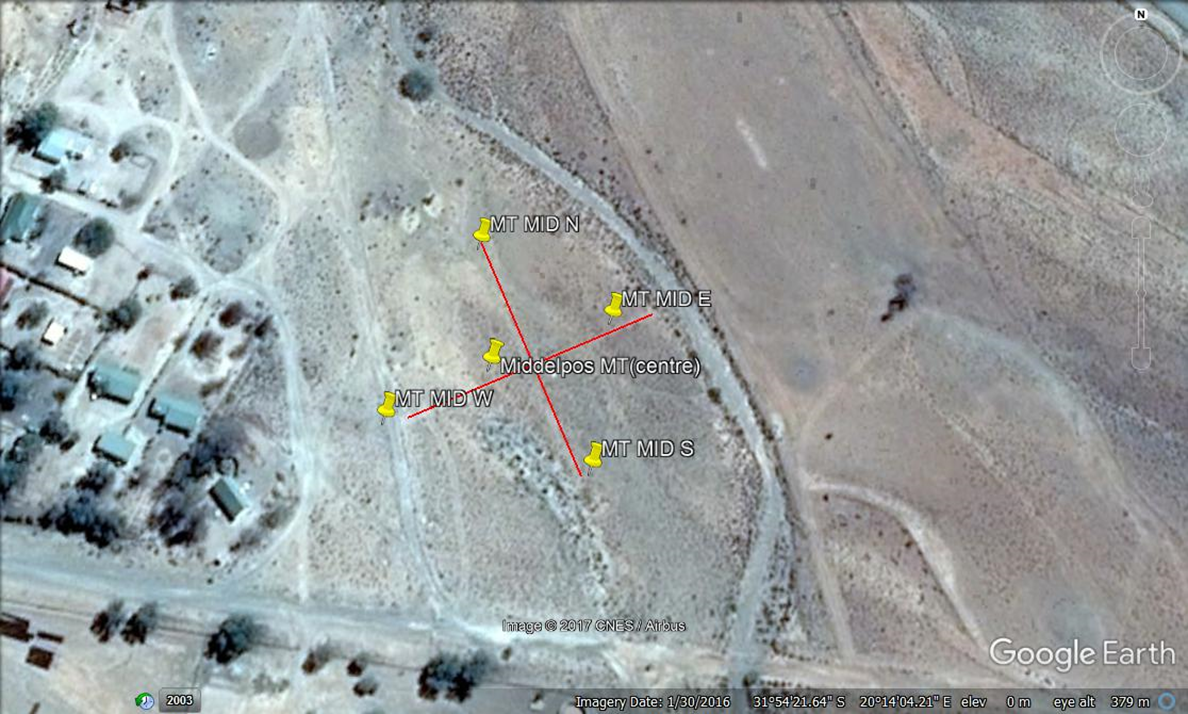
\includegraphics[width=\textwidth]{../figures/site.png}
  \caption{Layout of the MT instrumentation at Middelpos. MID N(orth), MID S(outh), MID E(ast), and MID W(est) indicate the locations of the electric field electrodes. The length of each electrode line is $100$~m. The LEMI-417 instrument is located at the crossing of the two electrode lines. The magnetometer is positioned $5$~m from the LEMI-417 to reduce the impact of instrument currents on its measurements.
}
 \label{fig:site}
\end{figure}

The time series of 1--second--cadence electric, $\mathbf{E}(t)$, and magnetic, $\mathbf{B}(t)$, field measurements is shown in Figure~\ref{fig:timeseries}. Each component $k=x \mbox{ or } y$ of $\mathbf{E}(t)$ was despiked by finding times when $|E_k(t+1)-E_k(t)|\ge 0.1$~mV/km and replacing values in the time range $[t-1, t+5]$ with linearly interpolated values based on $E_k(t-2)$ and $E_k(t+6)$. The number of spikes in $E_x(t)$ was $112$ ($0.002$\%); for $E_y(t)$, the number was $904$ ($0.02$\%).

The averaged amplitudes of the Fourier coefficients for each vector component of the time series shown in Figure~\ref{fig:timeseries}(a) are shown in Figure~\ref{fig:timeseries}(b). The averaged amplitudes shown are frequency--domain band average of the discrete Fourier transform amplitudes. The values of the band centers, marked with filled circles, the number of values in each band, and the band boundaries are given in Table~\ref{table:evalfreqs55d} of Appendix~\ref{appendix:tables}. The vertical bars correspond to 95\% confidence intervals; the length of the confidence interval for the magnitude of a Fourier coefficient, $\Delta|\widetilde{A}|$, calculated using propagation of errors in $|\widetilde{A}| = \sqrt{A_\text{r}^2 + A_\text{i}^2}$, is

\begin{equation}
\Delta\big|\widetilde{A}\big| = \sqrt{(A_\text{r}\Delta A_\text{r})^2 + (A_\text{i}\Delta A_\text{i})^2} / \big|\widetilde{A}\big|
\end{equation}

\noindent
where $\Delta A_\text{r}$ and $\Delta A_\text{i}$ are the lengths of the 95\% confidence intervals for the real ($A_\text{r}$) and imaginary ($A_\text{i}$) parts of $\widetilde{A}$, respectively; $\widetilde{A}$ is one of the $\widetilde{B}_x$, $\widetilde{B}_y$, $\widetilde{E}_x$, and $\widetilde{E}_y$, which are frequency domain averages shown in Figure~\ref{fig:timeseries}(b). The lengths of the 95\% symmetric confidence intervals for the averages $A_\text{r}$ and $A_\text{i}$ were determined using $\pm 2 (s/\sqrt{n})t^{-1}_{n-1}(0.025)$, where $n$ is the number of values used to calculate the average, $t^{-1}_{n-1}(0.025)$ is the inverse $t$-distribution evaluated at $0.025$, and $s$ is the standard deviation of the sample.

\begin{figure}
     \subfigure[]{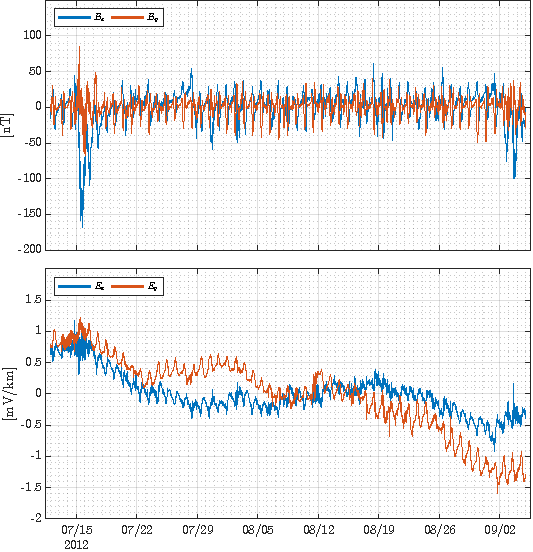
\includegraphics[width=0.45\textwidth]{../figures/tsplot-original-Middelpos-tf1.pdf}}
     \hspace{10pt}
     \subfigure[]{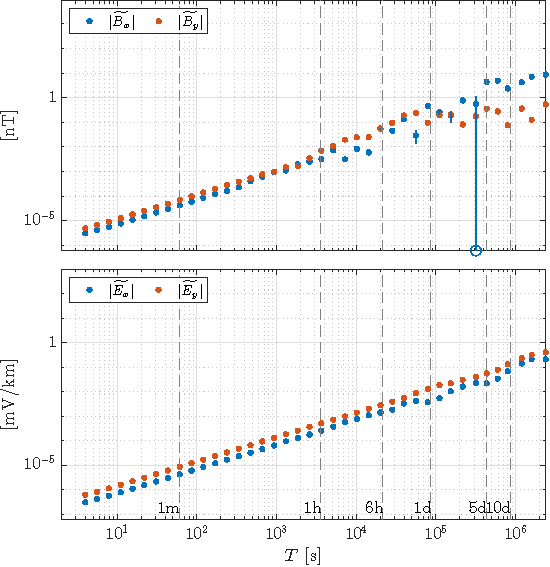
\includegraphics[width=0.45\textwidth]{../figures/dftplot-original-averaged-magnitudes-Middelpos-tf1.pdf}}
     \caption{(a) Measurements used for analysis after mean subtraction and despiking. (b) Magnitudes of discrete Fourier transform coefficients for measurements in (a). The vertical bars correspond to 95\% confidence intervals and a filled circle indicates the computed lower bound is below zero.}
  \label{fig:timeseries}
\end{figure}

\section{Models and Methods}
\label{section:Models_and_Methods}

$\mathbf{E}(t)$ and $\mathbf{B}(t)$ measurements are used to estimate the complex--valued transfer function matrix $\boldsymbol{\mathcal{\widetilde{Z}}}$ in

\begin{equation}
    \mathbf{\widetilde{E}}(f_e) = \boldsymbol{\mathcal{
\widetilde{Z}}}(f_e)\mathbf{\widetilde{B}}(f_e)\text{ ,}
\end{equation}

\noindent where $f_e$ is an ``evaluation frequency" and

\begin{equation}
    \boldsymbol{\mathcal{\widetilde{Z}}}(f_e) = 
        \begin{bmatrix}
            \widetilde{Z}_{xx}(f_e) & \widetilde{Z}_{xy}(f_e)\\
            \widetilde{Z}_{yx}(f_e) & \widetilde{Z}_{yy}(f_e)
        \end{bmatrix}
\end{equation}

\noindent using a method described by \cite{Sims1971}: for each $\mathbf{\widetilde{E}}$ vector component $k=x\mbox{ or }y$, a four parameter over--determined linear regression is performed using

\begin{equation}
  \widetilde{E}_k(f) = \widetilde{Z}_{kx}(f)\widetilde{B}_x(f) + \widetilde{Z}_{ky}(f)\widetilde{B}_y(f)
  \label{eqn:single}
\end{equation}

\noindent with values of $f$ in a band around $f_e$. (The number of parameters is four because the two regression parameters $\widetilde{Z}_{kx}$ and $\widetilde{Z}_{ky}$ in Equation~\ref{eqn:single} are complex--valued; the actual regression is performed using only real numbers -- see \cite{Egbert1986}). This regression method corresponds to minimizing the least-squared error between the predicted and measured $\widetilde{E}_k(f)$ values.

Historically, two methods have been used for computing the Fourier coefficients for uniform cadence time series -- one uses the standard DFT (Discrete Fourier Transform) formula for equally spaced records, typically implemented using the FFT algorithm. The other is an approximation based on the method of ``Cascade Decimation" \citep{Wight1980}, which can require less memory and produces logarithmically spaced evaluation frequencies. Here, we use the standard DFT formula because it is not an approximation and memory is not a constraint for the data considered.

There are two general methods for computing estimates of $\widetilde{Z}_{kx}$ and $\widetilde{Z}_{ky}$ for each evaluation frequency when there are not significant data gaps: (1) compute the Fourier coefficients using the full time series and then perform regression using the Fourier coefficients in a band centered on the evaluation frequency and (2) split the full time series into (possibly overlapping) segments, perform a regression on each segment using the Fourier coefficients in a band centered on the evaluation frequency to find segment estimates of $\widetilde{Z}_{kx}$ and $\widetilde{Z}_{ky}$, and then average the segment estimates of $\widetilde{Z}_{kx}$ and $\widetilde{Z}_{ky}$. In this paper, we present results from both methods; for the second method, non--overlapping time series segments were used, and the estimates of $\widetilde{Z}_{kx}$ and $\widetilde{Z}_{ky}$ are unweighted averages. 

A key result is that there are significant differences in the transfer functions computed using these two approaches. We have verified that the two approaches should give transfer functions without statistically significant differences by generating a simulated $\mathbf{E}(t)$ by convolving a white noise $\mathbf{B}(t)$ with a known transfer function $\boldsymbol{\mathcal{\widetilde{Z}}}$ $N$ times. The two approaches will not give identical transfer functions due to the differences in frequency grids, but the averaged and interpolated transfer functions for large $N$ converges. As a result, we conclude that the observed differences are likely due to non-stationarity.

In the literature, results are often presented using only one algorithm and a single set of parameters for that algorithm. However, it seems that, given that these two reasonable approaches for computing a transfer function can yield different results, there is an ``algorithmic uncertainty" that should be accounted for by computing the transfer function using different algorithms and varying parameter values for a given algorithm. There is also an uncertainty due to the data selection; \cite{Chen2022} noted that for some SAMTEX sites, the transfer functions were dependent on the time intervals used in their computation, in particular on whether the interval contained a period of high geomagnetic activity. This is expected because the plane wave approximation is invalid when geomagnetic activity is strong. Conversely, in the limit of low geomagnetic activity, the signal-to-noise ratio is low, leading to large error bars in the computed transfer functions.

There are two common modifications to these estimation methods. The first is the ``remote reference"  method, which uses $\mathbf{B}(t)$ measurements covering the same time interval from a nearby magnetometer~\citep{Simpson2005}. In our case, we do not have such measurements. The second uses a robust algorithm for regression, which involves computing estimates of $\widetilde{Z}_{kx}$ and $\widetilde{Z}_{ky}$ using a custom error function instead of the standard sum--of--squares error function (\cite{Simpson2005}; see also~\cite{Thomson2016} for a discussion about the ``overselling'' of this method). The custom error function automatically downweights outliers. For the data considered, we have found that this method produces differing results only at evaluation frequencies where the signal-to-prediction error is less than 1.0.

\section{Results}
\label{section:Results}

Figure~\ref{fig:z} shows the results of the regression described in Section~\ref{section:Models_and_Methods}. For the components of $\boldsymbol{\mathcal{\widetilde{Z}}}$ computed using one $55$--day segment, 95\% confidence intervals were computed using formulas that assume the regression errors are independent and identically distributed (\cite{Draper1981}; chapter 2.6). For the magnitudes calculated using the average of $55$ one--day segments, the 95\% confidence intervals were calculated using the formula given in Section~\ref{section:Data} for the magnitudes of the DFT amplitudes. The error bars for the phases were calculated using propagation of errors on

$$\phi_{ij} = \tan^{-1}[
  \text{Im}(\widetilde{Z}_{ij})
  /
  \text{Re}(\widetilde{Z}_{ij})],
$$

\noindent which gives

$$
  \Delta\phi_{ij} = (1/|\widetilde{Z}_{ij}|^2)
  \sqrt{
    \big[
      \text{Im}(\widetilde{Z}_{ij})\text{Re}(\Delta \widetilde{Z}_{ij})
    \big]^2
    +
    \big[
      \text{Re}(\widetilde{Z}_{ij})\text{Im}(\Delta \widetilde{Z}_{ij})
    \big]^2
  },
$$

\noindent
where $\Delta \widetilde{Z}_{ij}$ is the 95\% confidence interval length for element $\widetilde{Z}_{ij}$ of $\boldsymbol{\mathcal{\widetilde{Z}}}$, $|\boldsymbol{\cdotp}|$ is the complex magnitude, and $\text{Re}(\boldsymbol{\cdotp})$ and $\text{Im}(\boldsymbol{\cdotp})$ are the real and imaginary parts of the argument, respectively.

The quality of the computed transfer functions were assessed using the traditional coherence metric and also a signal--to--error metric.

The squared coherence, $\text{Coh}^2_{XY}(f_e)$, was computed using

\begin{equation}
  \text{Coh}^2_{XY}(f_e) = \frac{\left|\displaystyle\sum_{j=1}^{N_e}\widetilde{X}^*(f_j)\widetilde{Y}(f_j)\right|^2}{\displaystyle\sum_{j=1}^{N_e} \left|\widetilde{X}(f_j)\right|^2\sum_{j=1}^{N_e} \left|\widetilde{Y}(f_j)\right|^2},
\end{equation}

\noindent
where $j$ is the index of the DFT frequency in the band centered on $f_e=1/T_e$; Tables~\ref{table:evalfreqs55d} and~\ref{table:evalfreqs1d} in Appendix~\ref{appendix:tables} list the band centers, ranges, and number of frequencies, $N_e$, in each band for each regression method.

95\% confidence intervals were computed using bootstrap resampling: for each $f_e$ band, the $N_e$ pairs of $\widetilde{Z}_{kx}$ and $\widetilde{Z}_{ky}$ were randomly selected with replacement, and the sums in the $\text{Coh}$ formula were computed using these randomly selected pairs. This process was repeated $1,000$ times, and the results were sorted in ascending order; the maximum $\text{SE}$ error bar value is the $975$th value in the sorted list, and the minimum is the $25$th. No confidence intervals were computed if $N_e\le 10$.

Traditionally, the primary quality metric used for evaluating the transfer function is $\text{Coh}^2_{E_xB_y}$ and $\text{Coh}^2_{E_yB_x}$. A limitation of this metric is that it does not directly quantify how well the predicted electric field matches the measured electric field. It quantifies only the coherence between the measured quantities. As a result, we have also computed the coherence between the measured and predicted electric field, $\text{Coh}^2_{E_kE^\text{p}_k}$ ($k=x\mbox{ or }y$), as it is a more direct measure of the ability of the transfer function to reproduce the signal.

Although $\text{Coh}^2_{E_kE^\text{p}_k}$ is a more direct measure of how well a transfer function reproduces the measured electric field is still has a limitation --- two signals that are identical except for a scaling factor will have the same coherence for any scaling factor. As a result, we have introduced the signal--to--error, which can be used to make a more direct assessment of how well the estimated transfer function captures the measured signal.

The signal--to--error ratio, $\text{SE}_k(f_e)$, for component $k=x\mbox{ or }y$ of $\mathbf{E}$ was calculated using

\begin{equation}
\text{SE}_k(f_e) = \frac{\displaystyle\sum_{j=1}^{N_e} \left|\widetilde{E}_k(f_j)\right|^2}{\displaystyle\sum_{j=1}^{N_e}\left|\Delta\widetilde{E}_k(f_j)\right|^2},
\label{eqn:se}
\end{equation}

\noindent where the summation frequencies and $f_e$ values are the same as those used for computing the $\text{Coh}$.

The error, $\Delta\widetilde{E}_k = \widetilde{E}_k^{\text{p}}-\widetilde{E}_k$, is the difference between the complex--valued DFT amplitudes of the predicted, $E_k^\text{p}(t)$, and measured, $E_k(t)$, signals after convolution with a Parzen window. For both regression methods, the predicted signal, $E_k^{\text{p}}$, was computed by linearly interpolating the real and imaginary parts of $\widetilde{Z}_{kx}$ and $\widetilde{Z}_{ky}$ onto a uniform frequency grid of $N=86400\times 55$ points. At interpolation grid frequencies outside the range of $f_e$ values, the interpolated values of $\widetilde{Z}_{kx}$ and $\widetilde{Z}_{ky}$ were set to zero.

95\% error bars were computed using the same as method used for $\text{Coh}$. 

Note that $\text{SE}$ defined by Equation~\ref{eqn:se} differs in general from the signal--to--noise ratio, $\text{Coh}^2/(1-\text{Coh}^2)$ that applies only if the input signal and the noise in the output signal (which is unknown) are uncorrelated and the input signal has no noise (\cite{Miranda2006}; \cite{Pedersen1988}).

The squared coherence and signal-to-error associated with the transfer functions shown in Figure~\ref{fig:z} are shown in Figure~\ref{fig:se}. In the top panel of Figure~\ref{fig:se}(a), we see that the transfer function for $E_x$ only captures the variations in the data at periods longer than approximately 40 seconds, and that the model computed using one 55-day segment has a slightly higher $\text{SE}$ ratio. For $E_y$, the top panel of Figure~\ref{fig:se}(b) shows that the period range over which the transfer function produces useful predictions is from approximately 6 minutes to 6 hours.
%sxx = abs(sum(dftsegsx{s}.*conj(dftsegsx{s}),1));
%syy = abs(sum(dftsegsy{s}.*conj(dftsegsy{s}),1));
%sxy = abs(sum(conj(dftsegsx{s}).*dftsegsy{s},1));
%cxy(s,:) = sqrt(sxy/sqrt(sxx*syy));


\begin{figure}[h!]
  \vspace{-1.5em}
  \subfigure(a){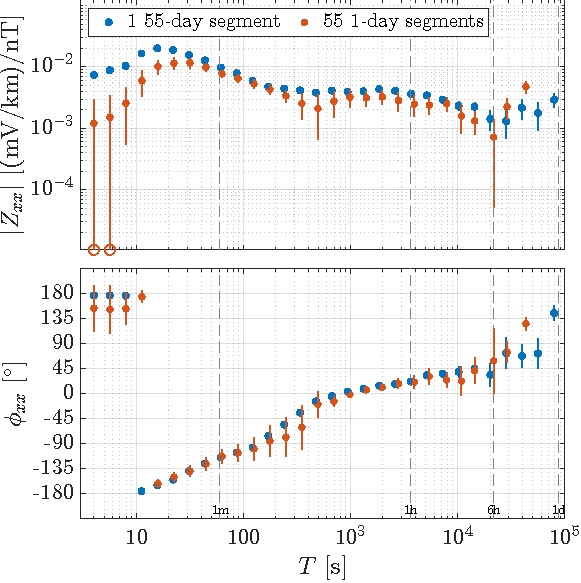
\includegraphics[width=0.48\textwidth]{../figures/zplot-magnitude_phase-Middelpos-tf1;Middelpos-tf3-Z_xx.pdf}} 
  \subfigure(b){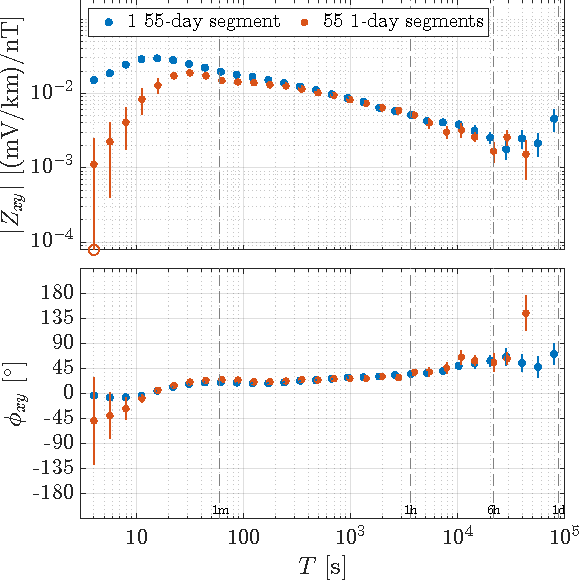
\includegraphics[width=0.48\textwidth]{../figures/zplot-magnitude_phase-Middelpos-tf1;Middelpos-tf3-Z_xy.pdf}} 
  \subfigure(c){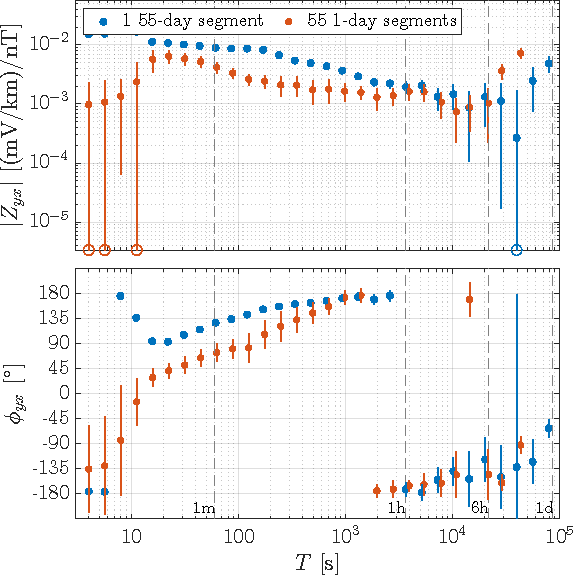
\includegraphics[width=0.48\textwidth]{../figures/zplot-magnitude_phase-Middelpos-tf1;Middelpos-tf3-Z_yx.pdf}} 
  \subfigure(d){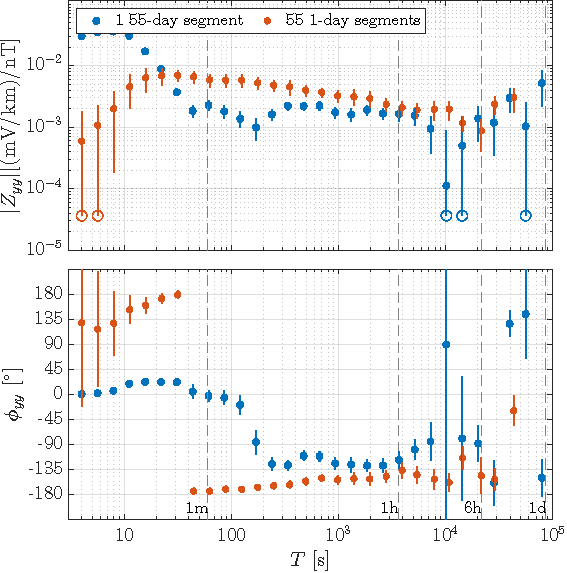
\includegraphics[width=0.48\textwidth]{../figures/zplot-magnitude_phase-Middelpos-tf1;Middelpos-tf3-Z_yy.pdf}} 

  \caption{Magnitudes and phases for components of $\boldsymbol{\mathcal{\widetilde{Z}}}$: (a) $|\widetilde{Z}_{xx}|$ and $\phi_{xx}$; (b) $|\widetilde{Z}_{xy}|$ and $\phi_{xy}$; (c) $|\widetilde{Z}_{yx}|$ and $\phi_{yx}$; and (d) $|\widetilde{Z}_{yy}|$ and $\phi_{yy}$. Open circles on the lower part of the impedance amplitude error bars indicate that this formula yielded a value below zero.}
  \label{fig:z}
\end{figure}
%The gray background in plots shown in Figure~\ref{fig:z} corresponds to periods for which the signal-to-prediction error, shown in Figure~\ref{fig:se}, is greater than unity.

\begin{figure}[h!]
  \subfigure(a){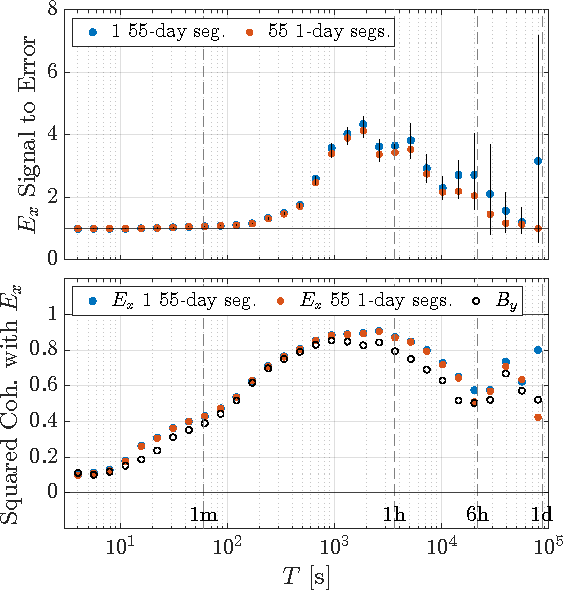
\includegraphics[width=0.48\textwidth]{../figures/snplot-Middelpos-tf1;Middelpos-tf3-E_x.pdf}} 
  \subfigure(b){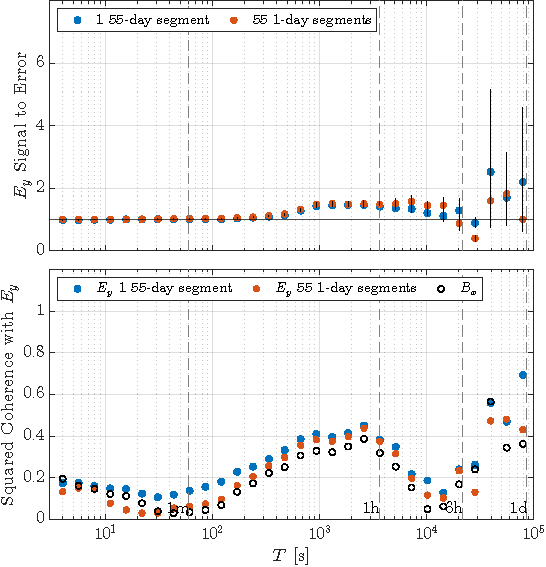
\includegraphics[width=0.48\textwidth]{../figures/snplot-Middelpos-tf1;Middelpos-tf3-E_y.pdf}} 

  \caption{Model metrics for (a) $E_x$, which depends on $\widetilde{Z}_{xx}$ and $\widetilde{Z}_{xy}$ shown in Figure~\ref{fig:z}(a)-(b) and (b) $E_y$, which depends on $\widetilde{Z}_{yx}$ and $\widetilde{Z}_{yy}$ shown in  Figure~\ref{fig:z}(b)-(c).}
  \label{fig:se}
\end{figure}

\clearpage

\section{Comparison to KAP103}

\cite{Jones2009} presented a summary of an MT survey of sites in South Africa; the results of the transfer function calculations are available from ~\cite{Jones2004}, which were computed using the Bounded Influence Remote Reference algorithm \citep{Chave2004}. The site nearest Middelpos is KAP103, which is shown in Figure~\ref{fig:map}.

In Figure~\ref{fig:timeseries-KAP103}, the 26--day magnetic and electric time series are shown along with the magnitude of their Fourier coefficients. The measurement interval included the large geomagnetic storm of November 20--22, 2003, that followed the October 31st ``Halloween" storm \citep{Gopalswamy2005}.

In Figure~\ref{fig:z-compare-KAP103}, we compare the pre--computed KAP103 transfer function (~\cite{Jones2004}) with that computed at Middelpos (corresponding to the ``1 55--day segment" lines shown in Figure~\ref{fig:z}). In addition, we have used the time series shown in Figure~\ref{fig:timeseries-KAP103} and the single transfer methodology described in the previous section.

There are several significant differences in the transfer functions shown in Figure~\ref{fig:z-compare-KAP103}. First, as in Figure~\ref{fig:z}, the method used to compute the transfer function can lead to statistically significant differences in the transfer functions (with respect to the computed error bars). In the case of the comparison of the BIRRP transfer functions with the single transfer function method used in the previous section, significant differences are found in all components of $\boldsymbol{\mathcal{\widetilde{Z}}}$, and these differences tend to occur at short and long periods.

Much larger differences exist between the amplitudes of the transfer functions computed at Middelpos and at KAP103, where the magnitudes of the Middelpos transfer function components range from 2 to 10 times smaller than those at KAP103. 

However, the transfer function phases are generally consistent, with the exception of $\widetilde{Z}_{yy}$.

To determine if the large geomagnetic storm may explain some of the differences, we have computed transfer functions using only data prior to November 20th and find consistent results, similar to \cite{Chen2022}, who found that for several of the SAMTEX sites, the computed transfer functions were not strongly dependent on whether the storm was included or not.

\begin{figure}[h]
\centering
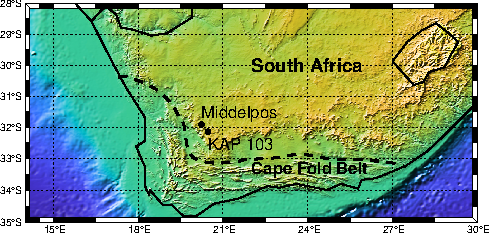
\includegraphics[width=\textwidth]{../figures/map.pdf}
\caption{Locations of Middelpos (Geographic [latitude, longitude] = [$-31.906^\circ$, $20.234^\circ$]) and KAP103 ([$-32.139^\circ$, $20.468^\circ$]) MT station. The relief map is from the ETOPO1 Global Relief Model (\cite{NCEI2006}), and the Cape Fold Belt line was derived from the digitization of Figure~1 of \cite{Nguuri2001}}.
\label{fig:map}
\end{figure}

%HER_lat=-34.4063;
%HER_lon=19.2687;
%HER_alt=65;  % m

\begin{figure}[h]
     \subfigure[]{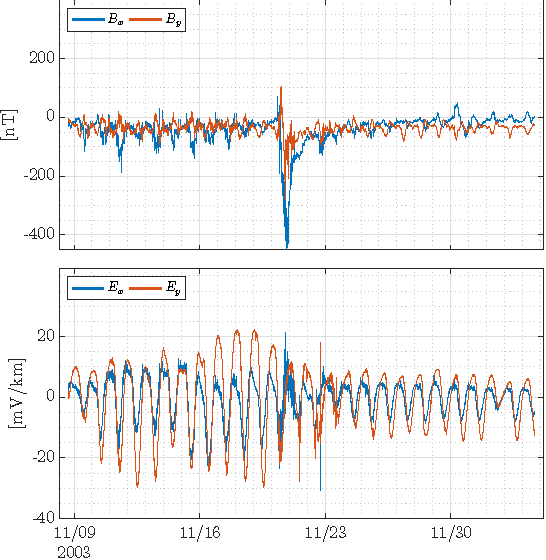
\includegraphics[width=0.45\textwidth]{../figures/tsplot-original-KAP103-tf1.pdf}}
     \hspace{10pt}
     \subfigure[]{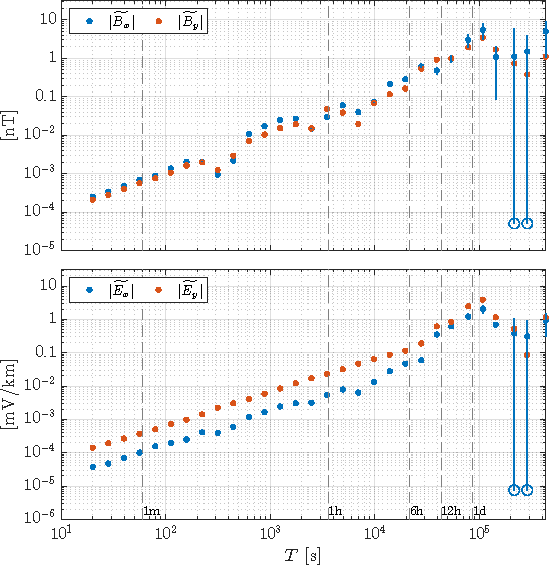
\includegraphics[width=0.45\textwidth]{../figures/dftplot-original-averaged-magnitudes-KAP103-tf1.pdf}}
     \caption{(a) Measurements used for analysis. (b) Magnitudes of discrete Fourier transform coefficients for measurements in (a). The vertical bars correspond to 95\% confidence intervals.}
  \label{fig:timeseries-KAP103}
\end{figure}

\clearpage


\begin{figure}[h!]
  \vspace{-2em}
  \subfigure(a){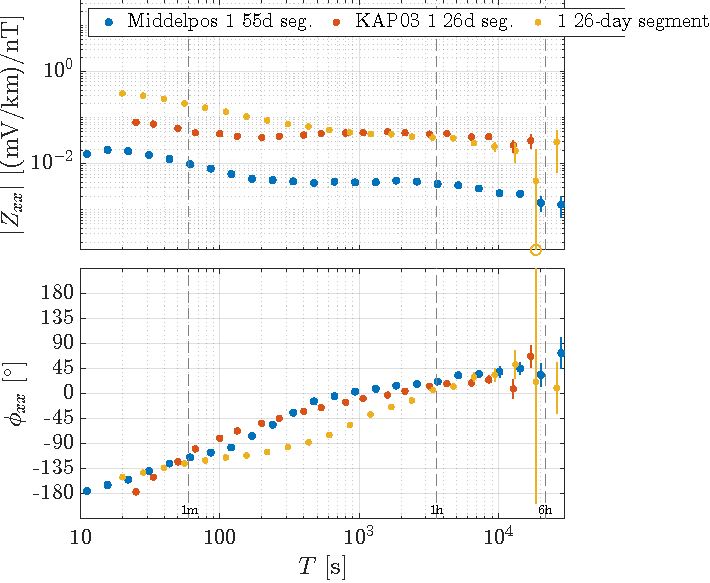
\includegraphics[width=0.48\textwidth]{../figures/zplot-magnitude_phase-Middelpos-tf1;KAP103-tf3;KAP103-tf1-Z_xx.pdf}} 
  \subfigure(b){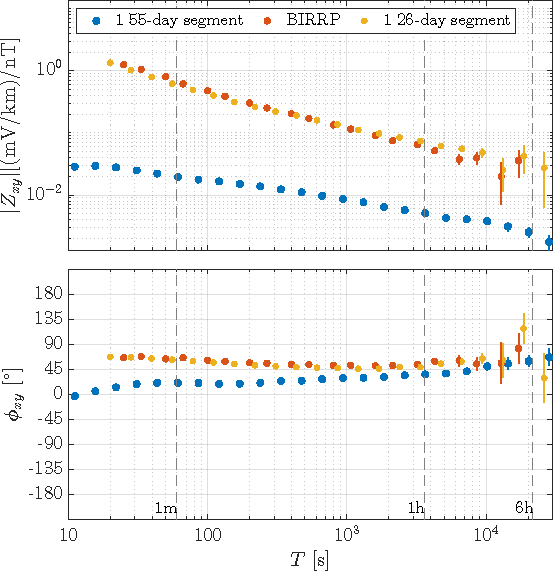
\includegraphics[width=0.48\textwidth]{../figures/zplot-magnitude_phase-Middelpos-tf1;KAP103-tf3;KAP103-tf1-Z_xy.pdf}} 
  \subfigure(c){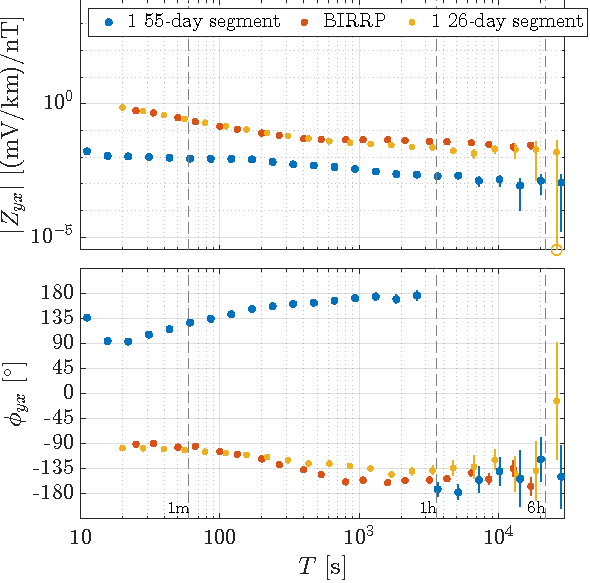
\includegraphics[width=0.48\textwidth]{../figures/zplot-magnitude_phase-Middelpos-tf1;KAP103-tf3;KAP103-tf1-Z_yx.pdf}} 
  \subfigure(d){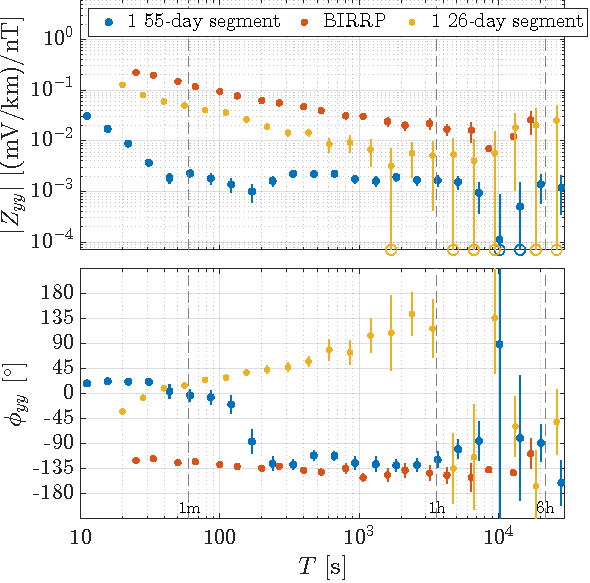
\includegraphics[width=0.48\textwidth]{../figures/zplot-magnitude_phase-Middelpos-tf1;KAP103-tf3;KAP103-tf1-Z_yy.pdf}} 

  \caption{Comparison of transfer function computed at Middelpos with two transfer functions computed at the KAP103 site. Error bars have the format as in Figure~\ref{fig:z}.}
  \label{fig:z-compare-KAP103}
\end{figure}

\section{Summary}

Transfer functions (surface impedances) were computed from magnetotelluric data collected at Middelpos, South Africa, over 55 days. We find that the computed transfer function depends on the method used to perform the regression. In one case, the full time range of data was split into 55 1-day segments, and the resulting 55 transfer functions were averaged in the frequency domain. In the other case, no splitting was performed, and a single transfer function was computed. At many frequencies, and for all components of the transfer function, differences were found that were inconsistent with the computed error bars. 

We also compared the transfer function at Middelpos with the nearest MT site from the SAMTEX campaign. The transfer function magnitudes differed significantly at all frequencies. 


\backmatter

\begin{appendices}

\clearpage

\section{The Middelpos MT Instrument}\label{appendix:instrument}

\begin{figure}[h]
  \centering
  (a)
  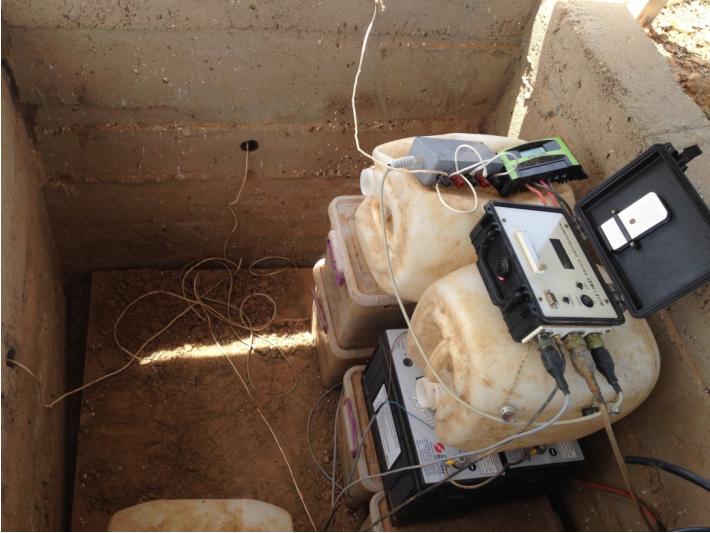
\includegraphics[width=0.45\textwidth]{../figures/instrument.pdf}
  (b)
  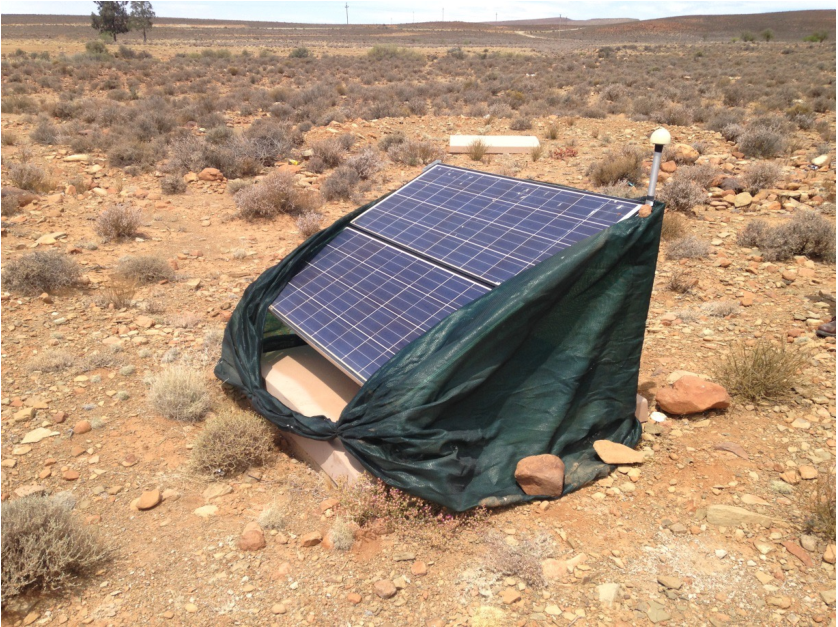
\includegraphics[width=0.45\textwidth]{../figures/solarpanel.pdf}
  \caption{\\
  The Middelpos MT instrument. (a) The LEMI-417 instrument and the 12~V lead-acid batteries that power it are in a subterranean enclosure with concrete walls. The instrument is mounted on two 25-liter water bottles to reduce temperature variation. (b) The solar panels are mounted on a steel frame over the enclosure. The side openings are covered with a canvas to prevent direct sunlight on the instrument. The small white dome above the solar panels is the GPS antenna.}
  \label{fig:lemi}
\end{figure}


\clearpage

\section{Evaluation Frequencies}\label{appendix:tables}

Band center frequencies (and periods), $f_e$ ($T_e$), lower and upper band bounds, $f_l$ and $f_u$ ($T_l$ and $T_u$), lower and upper band DFT indices, $i_l$ and $i_u$, and number of frequencies in band, $N_e$ for the 1-day and 55-day regression methods are shown in Tables~\ref{table:evalfreqs1d} and~\ref{table:evalfreqs55d}, respectively.


\begin{table}
  \caption{Frequency domain band information for the 55-day regression method.}
  \centering
  \small
  \input{../tables/Middelpos-tf3-evalfreq_table}
\label{table:evalfreqs55d}
\end{table}

\clearpage

\begin{table}[hbt]
  \caption{Frequency domain band information for the 1-day regression method.}
  \centering
  \small
  \input{../tables/Middelpos-tf1-evalfreq_table}
\label{table:evalfreqs1d}
\end{table}

\end{appendices}

%%===========================================================================================%%
%% If you are submitting to one of the Nature Portfolio journals, using the eJP submission   %%
%% system, please include the references within the manuscript file itself. You may do this  %%
%% by copying the reference list from your .bbl file, paste it into the main manuscript .tex %%
%% file, and delete the associated \verb+\bibliography+ commands.                            %%
%%===========================================================================================%%

\clearpage

\bibliography{../main}% common bib file
%% if required, the content of .bbl file can be included here once bbl is generated
%%\input sn-article.bbl

\end{document}
